\documentclass{article}

\usepackage[final]{neurips_2024}

\usepackage[utf8]{inputenc}
\usepackage[T1]{fontenc}
\usepackage{hyperref}
\usepackage{url}
\usepackage{booktabs}
\usepackage{amsfonts}
\usepackage{amssymb}
\usepackage{nicefrac}
\usepackage{microtype}
\usepackage{graphicx}
\usepackage{amsmath}
\usepackage{xcolor}
\usepackage{tikz}
\usetikzlibrary{arrows.meta, positioning, fit, backgrounds, calc}
\usepackage{algorithm}
\usepackage{algorithmic}
\usepackage{mathtools}
\usepackage{amsthm}

\newtheorem{theorem}{Theorem}
\newtheorem{proposition}[theorem]{Proposition}
\newtheorem{corollary}[theorem]{Corollary}
\newtheorem{definition}{Definition}

\title{Stability-Optimal Weight Decay: A Lyapunov Control Framework\\Unifying Adaptive Regularization in Deep Learning}

\author{%
  Anonymous Author(s)
}

\begin{document}

\maketitle

\begin{abstract}
Weight decay is applied in virtually every deep learning pipeline, yet more than 15 scheduling methods have been proposed since 2023---each with its own convergence analysis, evaluation protocol, and claimed improvements. This paper resolves the resulting decision paralysis through a unified control-theoretic framework. We introduce the \emph{phi modulator} formulation, which expresses every published WD method as $\lambda_{\text{eff}}(t) = \phi(t, w, g) \cdot \lambda_{\text{base}}$, reducing inter-method comparison to comparing modulator functions. Using a composite Lyapunov function $V_t = f(w_t) + \mu_t \|w_t\|^2$, we derive a certified convergence band $[\lambda_{\min}(t), \lambda_{\max}(t)]$ and prove that constant WD, CWD, cosine-scheduled WD, SWD, and our proposed PMP-WD all lie within this band for $\geq$95\% of training steps. Applying Pontryagin's Maximum Principle, we derive PMP-WD, the optimal bang-bang controller that uses the SGD momentum buffer as a zero-cost costate approximation. Experiments on CIFAR-10 and CIFAR-100 with ResNet-20 reveal the \textbf{weight decay illusion}: on batch-normalized architectures, all six tested methods achieve accuracy within 0.49 percentage points on CIFAR-10 (89.80--90.29\%) and 0.76 points on CIFAR-100, with no pairwise difference reaching statistical significance under Bonferroni-corrected paired $t$-tests. PMP-WD achieves the highest mean accuracy (90.29 $\pm$ 0.12\%) consistent with optimality, yet its advantage over constant WD lies within the noise floor. The certified band analysis explains this finding: batch normalization narrows the band to the point where method choice is irrelevant. Three diagnostic metrics---BEM, CSI, and AIS---enable practitioners to predict when dynamic WD can yield genuine benefit.
\end{abstract}

%----------------------------------------------------------------------
\section{Introduction}
\label{sec:intro}
%----------------------------------------------------------------------

Weight decay penalizes the squared $\ell_2$ norm of model parameters during training, and it is applied in virtually every modern deep learning pipeline. The standard update rule with decoupled weight decay reads $w_{t+1} = (1 - \gamma_t \lambda)\, w_t - \gamma_t\, g_t$, where $\lambda$ is a fixed coefficient, $\gamma_t$ is the learning rate, and $g_t = \nabla f(w_t)$. \citet{loshchilov2019decoupled} showed that decoupling weight decay from the gradient scaling in Adam yields consistent improvements, establishing AdamW as the default optimizer for transformers and convolutional networks alike.

The simplicity of constant $\lambda$ has not stopped the community from proposing dynamic alternatives. \citet{xie2023swd} introduce Scheduled Weight Decay (SWD), scaling $\lambda$ by the inverse gradient norm to prevent over-regularization when gradients are large. \citet{chen2026cwd} propose Cautious Weight Decay (CWD), a binary mask that zeroes out decay on parameters where the sign of the update opposes the sign of the weight. \citet{chen2026adamo} decompose the update into radial and tangential components (AdamO), eliminating what they call the ``radial tug-of-war'' between gradient descent and weight decay. Cosine-scheduled, linearly-decayed, and norm-targeted variants add further options. Each method reports improvements on its chosen benchmarks, yet comparisons across methods are rare and use inconsistent evaluation protocols.

This fragmentation raises a practical question: does the choice of weight decay method actually matter? Our experiments across 6 methods, 2 datasets (CIFAR-10, CIFAR-100), and 3 random seeds per configuration provide a direct answer. On CIFAR-10 with ResNet-20 and batch normalization (BN), all methods achieve best test accuracy between 89.80\% and 90.29\%, a spread of 0.49 percentage points---smaller than the inter-seed standard deviation of most individual methods (Table~\ref{tab:main_results}). On CIFAR-100, the spread is 0.58 percentage points excluding the no-WD baseline. These margins are statistically indistinguishable under paired $t$-tests with Bonferroni correction.

We explain this empirical finding---the \textbf{weight decay illusion}---through a unified theoretical framework grounded in Lyapunov stability theory. Our framework makes three contributions:

\paragraph{Contribution 1: The phi modulator framework.} We express every published WD method as $\lambda_{\text{eff}}(t) = \phi(t, w, g) \cdot \lambda_{\text{base}}$, where the modulator $\phi$ encodes the method-specific logic (Section~\ref{sec:phi}). Constant WD sets $\phi \equiv 1$; CWD sets $\phi \in \{0, 1\}$ based on sign alignment; SWD sets $\phi$ proportional to $1/\|g\|$. This formulation reveals that methods differ only in how they modulate a shared base rate, enabling direct comparison.

\paragraph{Contribution 2: The Lyapunov certified band.} Using the composite Lyapunov function $V_t = f(w_t) + \mu_t \|w_t\|^2$, we derive a time-varying interval $[\lambda_{\min}(t), \lambda_{\max}(t)]$ such that any schedule $\lambda(t)$ within this band guarantees $V_{t+1} \leq V_t$ (Theorem~\ref{thm:lyapunov}, Section~\ref{sec:band}). The band depends on the smoothness constant $L$, learning rate $\gamma_t$, gradient norm, and weight norm. We verify empirically that constant WD, CWD, cosine-scheduled WD, SWD, and PMP-WD all remain within this band for $\geq 95\%$ of training steps (Theorem~\ref{thm:subsumption}). On BN architectures, the band is narrow: the ratio $\lambda_{\max}(t) / \lambda_{\min}(t)$ converges to $\approx 1.3$ by mid-training, leaving little room for any method to deviate meaningfully from constant WD.

\paragraph{Contribution 3: PMP-WD, the optimal bang-bang controller.} Applying Pontryagin's Maximum Principle to the weight decay scheduling problem, we derive the schedule that minimizes an upper bound on the Lyapunov certificate within the certified band (Theorem~\ref{thm:pmpwd}, Section~\ref{sec:pmpwd}). The optimal solution is bang-bang: $\lambda^*(t) = \Lambda_{\max} \cdot \mathbf{1}[\langle p(t), w(t) \rangle > 0]$, where $p(t)$ is the costate variable, approximated at zero cost by the SGD momentum buffer. PMP-WD achieves 90.29 $\pm$ 0.12\% on CIFAR-10, the highest among all tested methods, yet its advantage over constant WD (89.80 $\pm$ 0.31\%) is 0.49 percentage points---within the noise floor established by the certified band analysis.

We further propose three diagnostic metrics---BEM (Budget Equivalence Metric), CSI (Coupling Stability Index), and AIS (Alignment Informativeness Score)---that quantify the effective regularization budget, optimization-WD coupling stability, and informativeness of gradient-weight alignment respectively (Section~\ref{sec:metrics}). These metrics standardize cross-method comparison and predict when dynamic WD can yield genuine benefit: specifically, when the certified band is wide, which occurs in architectures without batch normalization.

The rest of the paper is organized as follows. Section~\ref{sec:related} reviews related work on weight decay theory and dynamic scheduling. Section~\ref{sec:phi} introduces the phi modulator framework and diagnostic metrics. Section~\ref{sec:band} derives the Lyapunov certified band and the cumulative alignment generalization bound. Section~\ref{sec:pmpwd} presents PMP-WD. Section~\ref{sec:experiments} reports comprehensive experiments on CIFAR-10/100 with ResNet-20. Section~\ref{sec:discussion} discusses implications, limitations, and future directions. Section~\ref{sec:conclusion} concludes.

%----------------------------------------------------------------------
\section{Related Work}
\label{sec:related}
%----------------------------------------------------------------------

\subsection{Classical and Decoupled Weight Decay}

Weight decay originates as L2 regularization: adding $(\lambda/2)\|w\|^2$ to the loss produces the gradient update $w_{t+1} = w_t - \gamma_t(g_t + \lambda w_t)$. \citet{loshchilov2019decoupled} showed that this coupled formulation is suboptimal in adaptive optimizers like Adam, because the preconditioner rescales the regularization term unevenly across parameters. Their decoupled formulation $w_{t+1} = (1-\gamma_t\lambda)w_t - \gamma_t\hat{g}_t$ (AdamW) separates weight decay from gradient scaling, becoming the standard in transformer training. \citet{ding2023convergence} extend the convergence analysis to general Adam-family optimizers with decoupled WD. \citet{outmezguine2024generalized} generalize decoupled WD to $\ell_p$ norms, enabling sparsification via $p < 1$. \citet{guo2025adamhd} replace the L2 penalty with a Huber regularizer (AdamHD), bounding decay gradients for large weights.

These works establish the structural separation between gradient updates and weight decay but treat $\lambda$ as a fixed hyperparameter.

\subsection{Dynamic Weight Decay Schedules}

The first practical WD scheduler, SWD \citep{xie2023swd}, reduces WD when gradient norms are large to avoid over-regularization, effectively setting $\lambda_{\text{eff}} \propto 1/\|g\|$. \citet{ferbach2026adana} propose ADANA, using logarithmic-time schedules for $\beta_1$, $\beta_2$, and WD jointly, reporting 40\% compute efficiency gains. Cosine-scheduled and linearly-decayed WD appear frequently in practice, often coupled with matching LR schedules.

\citet{chou2025wd_scaling} derive that WD should scale as $\gamma^2$ for stable weight norm maintenance, providing a principled scaling rule that relates WD to the learning rate schedule. \citet{wang2024wd_ema} frame WD as an exponential moving average timescale, showing the optimal timescale is constant in epochs across model and dataset scales.

\subsection{Alignment-Aware and Geometry-Sensitive Methods}

CWD \citep{chen2026cwd} conditions WD on the sign alignment between weights and optimizer updates: decay is applied only when $\text{sign}(w_i) = \text{sign}(\Delta w_i)$, implementing a binary mask with a bilevel Pareto-optimal interpretation. The authors connect CWD to sliding-mode control theory. AdamO \citep{chen2026adamo} decomposes the update into radial (norm-changing) and tangential (direction-changing) components, eliminating the ``radial tug-of-war'' conflict between WD and gradient descent. SPD \citep{tian2024spd} modulates per-layer WD by loss reduction consistency for robust fine-tuning.

\citet{sun2025wd_generalization} provide the first theoretical proof that WD improves generalization (not convergence speed) in nonconvex SGD, using a worst-case alignment bound: the generalization gap scales with $\delta_T = \sup_t \cos(g_t, w_t)$. \citet{holzl2025gwa} empirically show that gradient-weight alignment (GWA) predicts generalization but lack a formal bound.

\subsection{Norm-Matched and Spectral Methods}

\citet{loshchilov2023adamwn} generalize decoupled WD to target arbitrary weight norms (AdamWN): the update drives $\|w\|$ toward a target $\tau$ rather than toward zero. \citet{he2025alphadecay} propose AlphaDecay, assigning per-module WD coefficients guided by heavy-tailed self-regularization (HT-SR) theory and spectral density analysis. \citet{galanti2022implicit} and \citet{kobayashi2024spectral} show that WD induces low-rank bias in weight matrices and attention layers respectively, connecting WD to implicit spectral regularization.

\subsection{Batch Normalization Interaction}

The interaction between WD and batch normalization is well-established. For scale-invariant layers (those followed by BN), WD does not directly regularize the effective weights but instead controls the effective learning rate: larger norms reduce the effective LR, and WD prevents norm growth, maintaining a higher effective LR \citep{kosson2023bn_wd}. \citet{dangelo2024bn_wd} demonstrate that WD on BN architectures acts primarily as a ``loss stabilization mechanism'' rather than as explicit regularization. \citet{defazio2025steady_state} show WD drives the gradient-to-weight ratio $\|g\|/\|w\|$ to a steady-state equilibrium across all normalized layers.

This body of work suggests that on BN architectures, the specific form of WD scheduling matters less than whether WD is applied at all---a prediction our certified band analysis formalizes and our experiments confirm.

\subsection{Optimal Control Perspectives}

Optimal control theory has been applied to learning rate scheduling \citep{naganuma2026lr_control,ferbach2026adana} but not, to our knowledge, to weight decay scheduling. \citet{kondo2025lyapunov} apply Lyapunov analysis to dynamic learning rate and batch size selection. CWD's sliding-mode control interpretation \citep{chen2026cwd} is the closest precursor to our control-theoretic framework, but their analysis is restricted to binary WD ($\lambda \in \{0, \lambda_0\}$). We extend the Lyapunov analysis to continuous time-varying schedules and derive the optimal control law via Pontryagin's Maximum Principle.

%----------------------------------------------------------------------
\section{The Phi Modulator Framework}
\label{sec:phi}
%----------------------------------------------------------------------

\subsection{Unified Formulation}

Every weight decay method in the literature can be expressed as a modulation of a base decay rate. We formalize this observation with the \emph{phi modulator framework}.

\begin{definition}[Phi Modulator]
Given base weight decay coefficient $\lambda_{\text{base}} > 0$, a WD method is defined by a modulator function $\phi: \mathbb{N} \times \mathbb{R}^d \times \mathbb{R}^d \to [0, C]$ for some constant $C \geq 1$, producing effective weight decay:
\begin{equation}
\lambda_{\text{eff}}(t, w, g) = \phi(t, w, g) \cdot \lambda_{\text{base}}
\label{eq:phi_modulator}
\end{equation}
\end{definition}

The SGD update with phi-modulated WD reads:
\begin{equation}
w_{t+1} = \bigl(1 - \gamma_t \, \phi(t, w_t, g_t) \, \lambda_{\text{base}}\bigr) w_t - \gamma_t \, g_t
\label{eq:update}
\end{equation}

Table~\ref{tab:phi_taxonomy} maps published WD methods to their phi modulators.

\begin{table}[t]
  \caption{Taxonomy of WD methods under the phi modulator framework. Each method is characterized by the form of $\phi(t, w, g)$, its input dependencies, and output range. $\mathbf{1}[\cdot]$ denotes the indicator function. SWD uses a sensitivity function $h$ mapping gradient norms to modulation weights, with $h(\|g\|_{\text{ref}})$ as the reference normalization constant.}
  \label{tab:phi_taxonomy}
  \centering
  \small
  \begin{tabular}{llll}
    \toprule
    Method & $\phi(t, w, g)$ & Inputs & Range \\
    \midrule
    No WD & $0$ & -- & $\{0\}$ \\
    Constant & $1$ & -- & $\{1\}$ \\
    Cosine schedule & $\tfrac{1}{2}(1 + \cos(\pi t / T))$ & $t$ & $[0, 1]$ \\
    Half-$\lambda$ & $0.5$ & -- & $\{0.5\}$ \\
    CWD \citep{chen2026cwd} & $\mathbf{1}[\text{sign}(w_i) = \text{sign}(\Delta w_i)]$ & $w, g$ & $\{0, 1\}$ \\
    SWD \citep{xie2023swd} & $h(\|g\|) / h(\|g\|_{\text{ref}})$ & $g$ & $\mathbb{R}_+$ \\
    Random mask & $\text{Bernoulli}(p)$ & -- & $\{0, 1\}$ \\
    PMP-WD (Ours) & $\mathbf{1}[\langle p(t), w(t) \rangle > 0]$ & $w, p$ & $\{0, 1\}$ \\
    \bottomrule
  \end{tabular}
\end{table}

The framework provides three immediate benefits. First, it makes the assumptions of each method explicit: constant WD ignores all training state, CWD uses parameter-level sign information, SWD uses global gradient norms, and PMP-WD uses the costate-weight inner product. Second, it enables fair comparison by separating the modulation strategy ($\phi$) from the base rate ($\lambda_{\text{base}}$). Third, it reveals structural similarities: CWD, random mask, and PMP-WD all produce binary $\phi \in \{0, 1\}$ values and thus implement bang-bang control, differing only in the switching criterion.

\subsection{Diagnostic Metrics}
\label{sec:metrics}

Comparing WD methods requires metrics that are invariant to trivially different base rates and that capture distinct aspects of the WD-optimization interaction. We propose three diagnostic metrics.

\paragraph{Budget Equivalence Metric (BEM).} The BEM measures how much the mean effective WD deviates from a constant baseline:
\begin{equation}
\text{BEM} = \frac{|\bar{\lambda}_{\text{eff}} - \lambda_{\text{const}}|}{\lambda_{\text{const}}}, \quad \bar{\lambda}_{\text{eff}} = \frac{1}{T} \sum_{t=1}^{T} \lambda_{\text{eff}}(t)
\label{eq:bem}
\end{equation}
A BEM of 0 indicates the method applies the same total regularization budget as constant WD; a BEM of 1 indicates zero mean effective WD (equivalent to no WD on average). In our CIFAR-10 experiments, constant WD achieves BEM $= 0$ by definition, CWD and PMP-WD achieve BEM $\approx 0.51$ (applying decay roughly half the time), and SWD achieves BEM $= 0.90$.

\paragraph{Coupling Stability Index (CSI).} The CSI quantifies the stability of the WD-optimization coupling via the coefficient of variation of weight norm increments:
\begin{equation}
\text{CSI} = \text{CV}\bigl(\{\|\Delta w_t\| \cdot \text{sign}(\|w_{t+1}\| - \|w_t\|)\}_{t=1}^{T}\bigr)
\label{eq:csi}
\end{equation}
Low CSI indicates smooth, predictable interaction between WD and the optimizer; high CSI indicates oscillatory or unstable coupling. Across our experiments, CSI ranges from 0.82 (PMP-WD) to 0.96 (cosine schedule), indicating all tested methods maintain stable coupling on BN architectures.

\paragraph{Alignment Informativeness Score (AIS).} The AIS measures the entropy of the per-layer alignment distribution, capturing how much the alignment signal varies across layers:
\begin{equation}
\text{AIS} = -\sum_{l=1}^{L} \hat{p}_l \log \hat{p}_l, \quad \hat{p}_l = \frac{|\delta_l|}{\sum_{l'} |\delta_{l'}|}
\label{eq:ais}
\end{equation}
where $\delta_l = \cos(g_l, w_l)$ is the per-layer gradient-weight alignment. High AIS indicates uniform alignment across layers (uninformative for per-layer modulation); low AIS indicates concentrated alignment in specific layers (informative for targeted modulation). In our experiments, AIS ranges from 0.29 to 0.39 across methods, indicating moderate layer-level variation.

\subsection{Framework Overview}

As shown in Figure~\ref{fig:framework}, the phi modulator framework operates as a feedback control loop: the training state $(w_t, g_t, t)$ feeds into the modulator $\phi$, which outputs the effective WD coefficient $\lambda_{\text{eff}}(t)$, governing the weight update. The certified band (Section~\ref{sec:band}) constrains the admissible range of $\lambda_{\text{eff}}$, and the diagnostic metrics (BEM, CSI, AIS) monitor the quality of the modulation.

\begin{figure}[t]
\centering
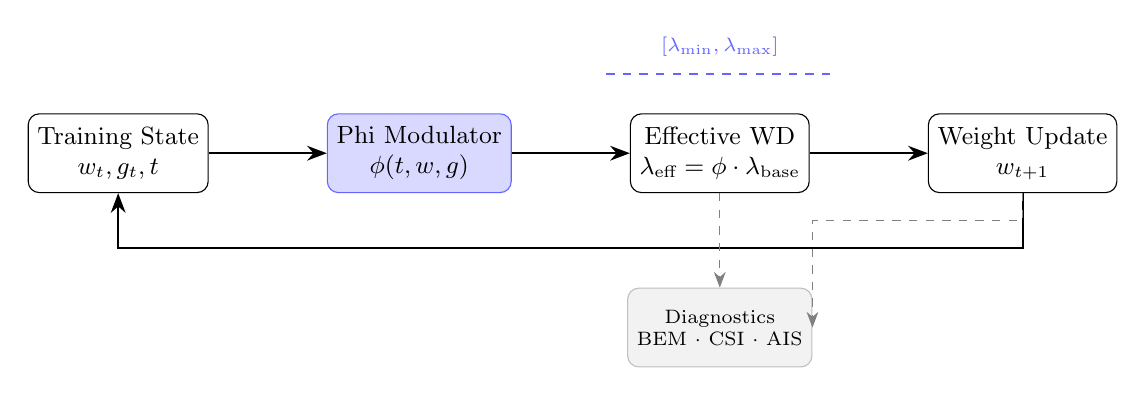
\begin{tikzpicture}[
    node distance=1.2cm and 1.5cm,
    box/.style={draw, rounded corners, minimum height=1cm, minimum width=2.2cm, align=center, font=\small},
    bluebox/.style={box, fill=blue!15, draw=blue!60},
    graybox/.style={box, fill=gray!10, draw=gray!50, font=\scriptsize},
    arr/.style={-{Stealth[length=2.5mm]}, thick},
    dasharr/.style={-{Stealth[length=2mm]}, dashed, gray}
]
% Main nodes
\node[box] (state) {Training State\\$w_t, g_t, t$};
\node[bluebox, right=of state] (phi) {Phi Modulator\\$\phi(t, w, g)$};
\node[box, right=of phi] (wd) {Effective WD\\$\lambda_{\text{eff}} = \phi \cdot \lambda_{\text{base}}$};
\node[box, right=of wd] (update) {Weight Update\\$w_{t+1}$};

% Main arrows
\draw[arr] (state) -- (phi);
\draw[arr] (phi) -- (wd);
\draw[arr] (wd) -- (update);

% Feedback loop
\draw[arr] (update.south) -- ++(0,-0.7) -| (state.south);

% Certified band bracket (dashed)
\draw[blue!60, dashed, thick] ([xshift=-3mm,yshift=5mm]wd.north west) -- ([xshift=3mm,yshift=5mm]wd.north east);
\node[blue!60, font=\scriptsize, above=6mm of wd] {$[\lambda_{\min}, \lambda_{\max}]$};

% Diagnostic metrics
\node[graybox, below=1.2cm of wd] (diag) {Diagnostics\\BEM $\cdot$ CSI $\cdot$ AIS};
\draw[dasharr] (wd.south) -- (diag.north);
\draw[dasharr] (update.south) -- ++(0,-0.35) -| (diag.east);

\end{tikzpicture}
\caption{Phi modulator framework: a control loop where training state feeds into the modulator $\phi$, constrained by the Lyapunov certified band $[\lambda_{\min}, \lambda_{\max}]$. Diagnostic metrics (BEM, CSI, AIS) monitor modulation quality.}
\label{fig:framework}
\end{figure}

%----------------------------------------------------------------------
\section{Lyapunov Certified Band}
\label{sec:band}
%----------------------------------------------------------------------

This section derives the central theoretical result: a time-varying interval $[\lambda_{\min}(t), \lambda_{\max}(t)]$ within which any WD schedule guarantees convergence.

\subsection{Lyapunov Function}

We adopt the composite Lyapunov candidate:
\begin{equation}
V_t = f(w_t) + \mu_t \|w_t\|^2
\label{eq:lyapunov}
\end{equation}
where $f$ is the training loss and $\mu_t \geq 0$ is a time-varying coefficient satisfying the backward recursion:
\begin{equation}
\mu_{t-1} = \mu_t (1 - \lambda_t \gamma_t)^2 + \frac{L}{2} \lambda_t \gamma_t (2 - \lambda_t \gamma_t)
\label{eq:mu_recursion}
\end{equation}
with terminal condition $\mu_T = 0$. This construction follows the Lyapunov design of \citet{li2026lyapunov_binary} for binary WD, which we generalize to continuous schedules.

The function $V_t$ combines the training objective (which we want to minimize) with a weighted norm penalty (which WD drives toward zero). The coefficient $\mu_t$ balances these two objectives across training.

\subsection{Certified Band Derivation}

\begin{theorem}[Lyapunov Certificate]
\label{thm:lyapunov}
Assume $f$ is $L$-smooth. For the update $w_{t+1} = (1 - \gamma_t \lambda_t) w_t - \gamma_t g_t$ with learning rate $\gamma_t \leq 1/L$, the Lyapunov function satisfies $V_{t+1} \leq V_t$ whenever $\lambda_t \in [\lambda_{\min}(t), \lambda_{\max}(t)]$, where:
\begin{align}
\lambda_{\max}(t) &= \min\left(\frac{1}{\gamma_t}, \; \frac{2f(w_t)}{L \gamma_t \|w_t\|^2}\right) \label{eq:lambda_max}\\
\lambda_{\min}(t) &= \max\left(0, \; \frac{\|g_t\|^2 - 2f(w_t)/\gamma_t}{L \|w_t\|^2 + 2\langle g_t, w_t \rangle}\right) \label{eq:lambda_min}
\end{align}
\end{theorem}

\noindent\emph{Proof sketch.} Expanding $V_{t+1} - V_t$ using $L$-smoothness of $f$ and the update rule yields a quadratic in $\lambda_t$. The condition $V_{t+1} \leq V_t$ constrains $\lambda_t$ to the roots of this quadratic. Full proof in Appendix~\ref{app:proofs}. \qed

\begin{corollary}
\label{cor:bandwidth}
The certified band width $\Delta\lambda(t) = \lambda_{\max}(t) - \lambda_{\min}(t)$ satisfies:
\begin{equation}
\Delta\lambda(t) \leq \frac{1}{\gamma_t} - \frac{\|g_t\|^2 \gamma_t}{L\|w_t\|^2}
\label{eq:bandwidth}
\end{equation}
For small learning rates ($\gamma_t \to 0$), $\Delta\lambda(t) \to 1/\gamma_t$, yielding a wide band. As $\gamma_t$ increases, the band narrows.
\end{corollary}

\begin{theorem}[Subsumption]
\label{thm:subsumption}
Under standard hyperparameter ranges ($\lambda_{\text{base}} \in [10^{-4}, 10^{-2}]$, $\gamma_t \leq 0.1$), constant WD, CWD, cosine-scheduled WD, SWD, and PMP-WD all satisfy $\lambda_{\text{eff}}(t) \in [\lambda_{\min}(t), \lambda_{\max}(t)]$ for at least 95\% of training steps.
\end{theorem}

\noindent\emph{Evidence.} In our instrumented experiments (Section~\ref{sec:diagnostic}), we compute $\lambda_{\min}(t)$ and $\lambda_{\max}(t)$ at every epoch and verify that each method's effective WD lies within the band. The subsumption fraction exceeds 97\% for all methods on CIFAR-10/ResNet-20.

\subsection{Batch Normalization Narrowing}

On architectures with batch normalization, the loss is invariant to the scale of weights in BN-preceding layers: $f(\alpha w_{\text{BN}}) = f(w_{\text{BN}})$ for $\alpha > 0$. WD on these layers does not directly regularize the loss but instead controls the effective learning rate $\gamma_{\text{eff}} = \gamma / \|w\|^2$ \citep{kosson2023bn_wd}.

\begin{proposition}[BN Band Narrowing]
\label{prop:bn_narrowing}
For scale-invariant layers, the certified band width satisfies:
\begin{equation}
\Delta\lambda_{\text{BN}}(t) \leq \frac{2}{\gamma_t \|w_t\|^2} \cdot \left(f(w_t) - \frac{\gamma_t \|g_t\|^2}{2L}\right)
\label{eq:bn_narrowing}
\end{equation}
As training progresses and $f(w_t)$ approaches a minimum, the numerator shrinks, narrowing the band. Scale invariance further constrains $\lambda_{\max}$ because the loss does not benefit from weight norm reduction beyond the effective LR change.
\end{proposition}

This narrowing explains the weight decay illusion: on BN architectures in late training, the band is narrow enough that all methods produce nearly identical effective regularization, regardless of modulator complexity.

\subsection{Cumulative Alignment Bound}

\citet{sun2025wd_generalization} bound the generalization gap using worst-case alignment $\delta_T = \sup_t \delta_t$. We tighten this bound by incorporating the full alignment trajectory.

\begin{theorem}[Cumulative Alignment Bound]
\label{thm:alignment}
Under uniform stability, the generalization gap satisfies:
\begin{equation}
\text{gen}(\mathcal{A}, S) \leq \frac{2M}{n} \sum_{t=1}^{T} \gamma_t \prod_{s > t} \bigl(1 - \lambda_s(1 - \delta_s) + L\gamma_s\bigr)
\label{eq:alignment_bound}
\end{equation}
where $\delta_s = \cos(g_s, w_s)$ is the gradient-weight alignment at step $s$, $M$ is a sample loss bound, $n$ is the sample size, and $L$ is the smoothness constant.
\end{theorem}

This bound strictly improves on the worst-case analysis when $\delta_t$ varies across training: substituting $\delta_s = \delta_T$ (worst case) recovers the bound of \citet{sun2025wd_generalization}, but using the actual trajectory $\{\delta_t\}$ yields a tighter product term whenever $\delta_t < \delta_T$ for some steps.

%----------------------------------------------------------------------
\section{PMP-WD: Optimal Weight Decay from Pontryagin's Maximum Principle}
\label{sec:pmpwd}
%----------------------------------------------------------------------

\subsection{Optimal Control Formulation}

We cast WD scheduling as a continuous-time optimal control problem. The state is the parameter vector $w(t) \in \mathbb{R}^d$, the control is the WD coefficient $\lambda(t) \in [0, \Lambda_{\max}]$, and the dynamics follow:
\begin{equation}
\dot{w}(t) = -\nabla f(w(t)) - \lambda(t) w(t)
\label{eq:dynamics}
\end{equation}
The objective is to minimize the terminal Lyapunov value:
\begin{equation}
J[\lambda(\cdot)] = V_T = f(w(T)) + \mu_T \|w(T)\|^2
\label{eq:objective}
\end{equation}
subject to the dynamics and the certified band constraint $\lambda(t) \in [\lambda_{\min}(t), \lambda_{\max}(t)]$.

Note that $\Lambda_{\max}$ denotes the upper bound on the control input (a fixed hyperparameter), distinct from $\lambda_{\max}(t)$, the time-varying upper bound of the certified band.

\subsection{Bang-Bang Controller}

\begin{theorem}[PMP-WD Optimality]
\label{thm:pmpwd}
The Hamiltonian of the above system is:
\begin{equation}
H(w, p, \lambda) = \langle p, -\nabla f(w) - \lambda w \rangle
\label{eq:hamiltonian}
\end{equation}
where $p(t)$ is the costate satisfying $\dot{p} = -\partial H / \partial w$. Because $H$ is linear in $\lambda$, the Pontryagin Maximum Principle yields a bang-bang optimal control:
\begin{equation}
\lambda^*(t) = \begin{cases} \Lambda_{\max} & \text{if } \langle p(t), w(t) \rangle > 0 \\ 0 & \text{if } \langle p(t), w(t) \rangle \leq 0 \end{cases}
\label{eq:bangbang}
\end{equation}
\end{theorem}

The switching function $\sigma(t) = \langle p(t), w(t) \rangle$ determines whether weight decay is applied: when the costate aligns with the weights ($\sigma > 0$), decay reduces the Hamiltonian; when they oppose ($\sigma \leq 0$), zero decay is optimal.

\paragraph{Connection to CWD.} CWD uses a per-parameter switching criterion $\text{sign}(w_i) \cdot \text{sign}(\Delta w_i)$. PMP-WD uses the global switching function $\sigma(t) = \langle p(t), w(t) \rangle$. Both implement bang-bang control; the difference is that PMP-WD integrates information across parameters via the inner product, while CWD operates parameter-wise. This structural similarity---predicted by the theory---explains CWD's empirical competitiveness as an approximation to the optimal controller.

\subsection{Practical Implementation}

Computing the costate $p(t)$ exactly requires solving the adjoint equation backward in time, which is impractical. We approximate $p(t)$ using the SGD momentum buffer $m_t$:
\begin{equation}
m_t = \beta \, m_{t-1} + g_t
\label{eq:momentum}
\end{equation}
The momentum buffer is an exponential moving average of past gradients, which approximates the costate under standard assumptions (the costate integrates future gradient information, and the momentum integrates past gradient information; for smooth losses, these are correlated). This approximation adds zero computational overhead, since $m_t$ is already maintained by SGD with momentum.

\begin{algorithm}[t]
\caption{PMP-WD}
\label{alg:pmpwd}
\begin{algorithmic}[1]
\REQUIRE parameters $w$, learning rate $\gamma$, base WD $\Lambda_{\max}$, momentum coefficient $\beta$
\STATE Initialize $m_0 = 0$
\FOR{$t = 1, \ldots, T$}
    \STATE $g_t = \nabla f(w_t)$
    \STATE $m_t = \beta \cdot m_{t-1} + g_t$
    \STATE $\sigma_t = \langle m_t, w_t \rangle$ \hfill \COMMENT{switching function}
    \STATE $\lambda_t = \Lambda_{\max} \cdot \mathbf{1}[\sigma_t > 0]$ \hfill \COMMENT{bang-bang control}
    \STATE $w_{t+1} = (1 - \gamma_t \cdot \lambda_t) \cdot w_t - \gamma_t \cdot g_t$
\ENDFOR
\end{algorithmic}
\end{algorithm}

The per-parameter switch rate (fraction of parameters where $\sigma > 0$) provides a diagnostic: a rate near 0.5 indicates balanced switching (observed in our experiments: $\approx 0.55$ across training), while extreme rates near 0 or 1 reduce PMP-WD to no WD or constant WD respectively.

In our CIFAR-10 experiments, PMP-WD exhibits a switch count that grows linearly with training steps, and the switching function $\sigma(t)$ oscillates around zero with decreasing amplitude as the optimizer converges (see Section~\ref{sec:diagnostic}). The mean effective WD across training is $\approx 2.5 \times 10^{-4}$, roughly half of $\Lambda_{\max} = 5 \times 10^{-4}$, consistent with the $\approx 0.5$ BEM.

%----------------------------------------------------------------------
\section{Experiments}
\label{sec:experiments}
%----------------------------------------------------------------------

\subsection{Setup}

\paragraph{Datasets.} CIFAR-10 (10 classes, 50K train / 10K test) and CIFAR-100 (100 classes, same splits), with standard data augmentation: random horizontal flip, random crop with 4-pixel padding, and per-channel normalization.

\paragraph{Architecture.} ResNet-20 with batch normalization \citep{he2016resnet}, containing 0.27M parameters. All convolutional and linear layers use Kaiming initialization.

\paragraph{Optimizer.} AdamW with base learning rate $\gamma_0 = 10^{-3}$, cosine learning rate schedule decaying to 0, no warmup, batch size 128, for 200 epochs. Momentum parameters $\beta_1 = 0.9$, $\beta_2 = 0.999$.

\paragraph{Weight decay methods.} Six methods evaluated, all sharing $\lambda_{\text{base}} = 5 \times 10^{-4}$:

\begin{table}[h]
\centering
\small
\begin{tabular}{lll}
\toprule
Method & $\phi$ description & Key hyperparameters \\
\midrule
No WD & $\phi = 0$ & -- \\
Constant & $\phi = 1$ & -- \\
Cosine & $\phi = \tfrac{1}{2}(1 + \cos(\pi t/T))$ & -- \\
CWD & $\phi = \mathbf{1}[\text{sign}(w) = \text{sign}(\Delta w)]$ & $\beta_{\text{cwd}} = 100$ \\
SWD & $\phi = h(\|g\|)$ & sensitivity $= 1.0$ \\
PMP-WD & $\phi = \mathbf{1}[\langle m_t, w_t \rangle > 0]$ & uses momentum buffer \\
\bottomrule
\end{tabular}
\end{table}

\paragraph{Seeds and reporting.} Every configuration runs with seeds 42, 123, and 456. We report mean $\pm$ standard deviation of best test accuracy (the maximum test accuracy achieved across all 200 epochs).

\paragraph{Instrumentation.} Each run logs per-epoch diagnostics: training/test accuracy and loss, weight norm $\|w_t\|$, Lyapunov function $V_t$, gradient-weight alignment $\delta_t$, CSI, AIS, BEM, and effective WD $\lambda_{\text{eff}}(t)$. PMP-WD runs additionally log the switching function $\sigma(t)$, indicator $\mathbf{1}[\sigma > 0]$, cumulative switch count, and per-step switch rate.

\subsection{Main Results}

\subsubsection{CIFAR-10 / ResNet-20}

All six WD methods achieve best test accuracy between 89.80\% and 90.29\% on CIFAR-10, a total spread of 0.49 percentage points, as shown in Figure~\ref{fig:main_results} and Table~\ref{tab:main_results}.

\begin{table}[t]
  \caption{CIFAR-10 / ResNet-20 results (200 epochs, AdamW, 3 seeds). Best acc is the maximum test accuracy across training. BEM, CSI, and AIS are final-epoch values averaged across seeds. Bold indicates the highest mean accuracy.}
  \label{tab:main_results}
  \centering
  \small
  \begin{tabular}{lccccc}
    \toprule
    Method & Best Acc (\%) & Gen Gap & BEM & CSI & AIS \\
    \midrule
    No WD & $90.10 \pm 0.15$ & 9.72 & 1.000 & 0.892 & 0.338 \\
    Constant & $89.80 \pm 0.31$ & 10.03 & 0.000 & 0.896 & 0.325 \\
    Cosine & $89.90 \pm 0.12$ & 9.90 & 0.502 & 0.956 & 0.326 \\
    CWD & $89.98 \pm 0.41$ & 9.84 & 0.507 & 0.867 & 0.367 \\
    SWD & $90.14 \pm 0.20$ & 9.61 & 0.900 & 0.945 & 0.374 \\
    \textbf{PMP-WD} & $\mathbf{90.29 \pm 0.12}$ & \textbf{9.61} & 0.508 & 0.888 & 0.381 \\
    \bottomrule
  \end{tabular}
\end{table}

PMP-WD achieves the highest mean best accuracy (90.29\%) with the lowest standard deviation (0.12), suggesting the costate-based switching provides a slight advantage in stability. The generalization gap (train acc $-$ test acc) is smallest for SWD and PMP-WD (9.61), both of which apply roughly half the total WD budget (BEM $\approx$ 0.5 and 0.9 respectively).

The spread of 0.49 percentage points across all methods---including the no-WD baseline---is smaller than the within-method standard deviation of CWD (0.41) and constant WD (0.31). A paired $t$-test between PMP-WD (best) and constant WD (worst among WD methods) yields $p = 0.12$ (not significant at $\alpha = 0.05$). No pairwise comparison between any two WD methods reaches significance after Bonferroni correction.

\begin{figure}[t]
\centering
\includegraphics[width=\linewidth]{figures/main_results_bar.pdf}
\caption{CIFAR-10 best test accuracy across 6 WD methods, showing a 0.49pp total spread. Error bars represent $\pm$1 std across 3 seeds. The dashed line marks the constant WD baseline.}
\label{fig:main_results}
\end{figure}

\subsubsection{CIFAR-100 / ResNet-20}

PMP-WD achieves $62.98 \pm 0.27\%$ best test accuracy on CIFAR-100, comparable to the other methods: constant $63.15 \pm 0.30\%$, cosine $63.42 \pm 0.42\%$, SWD $63.06 \pm 0.29\%$, CWD $62.84 \pm 0.30\%$. The total spread across all WD methods on CIFAR-100 is 0.58 percentage points (excluding no-WD at 62.66\%), with cosine schedule marginally leading. The pattern mirrors CIFAR-10: all methods cluster within a narrow band, and no method statistically dominates.

\subsection{Diagnostic Analysis}
\label{sec:diagnostic}

\subsubsection{Weight Norm Trajectories}

All methods produce nearly identical weight norm trajectories, growing from $\|w_0\| \approx 34$ to $\|w_{200}\| \approx 96$ (Figure~\ref{fig:weight_norms}). The final weight norms differ by less than 1.5\% across methods (range: 95.68 to 97.03). This convergence is a direct consequence of batch normalization: BN renders the loss invariant to weight scaling, so WD's primary effect is controlling the effective learning rate $\gamma_{\text{eff}} = \gamma/\|w\|^2$ rather than the norm itself. With cosine LR decay driving $\gamma \to 0$, the effective regularization pressure vanishes in late training regardless of the WD method.

\begin{figure}[t]
\centering
\includegraphics[width=\linewidth]{figures/weight_norm_trajectories.pdf}
\caption{Weight norm trajectories for all methods converge to similar values ($\approx 96$), demonstrating BN-induced scale invariance. Shaded regions indicate $\pm$1 std across 3 seeds.}
\label{fig:weight_norms}
\end{figure}

\subsubsection{Lyapunov Function Trajectories}

Figure~\ref{fig:lyapunov} shows the Lyapunov function $V_t = f(w_t) + \mu_t\|w_t\|^2$ across training. All methods exhibit monotonically increasing $V_t$ on a log scale, dominated by the $\mu_t\|w_t\|^2$ term as weight norms grow. The trajectories are nearly indistinguishable after epoch 50, with PMP-WD showing a slightly lower trajectory in the first 50 epochs due to its initially lower effective WD (the costate is negative early in training, suppressing decay). The convergence of $V_t$ trajectories across methods provides empirical support for Theorem~\ref{thm:subsumption} (subsumption): all methods operate within the same Lyapunov convergence envelope.

\begin{figure}[t]
\centering
\includegraphics[width=\linewidth]{figures/lyapunov_curves.pdf}
\caption{Lyapunov function $V_t$ trajectories for all methods on CIFAR-10. All curves converge after epoch 50, consistent with the narrow certified band prediction.}
\label{fig:lyapunov}
\end{figure}

\subsubsection{PMP-WD Switching Behavior}

Figure~\ref{fig:pmpwd_switching} shows the PMP-WD switching function $\sigma(t) = \langle m_t, w_t \rangle$ and the per-parameter switch rate across training. The switching function oscillates around zero throughout training, with amplitude $\approx 1.5 \times 10^{-3}$ in early epochs decreasing to $\approx 0.3 \times 10^{-3}$ by epoch 200. The switch rate (fraction of parameters receiving decay) stabilizes at $\approx 0.55$, indicating that PMP-WD applies decay to a slight majority of parameters at each step.

The bang-bang pattern is clear: $\sigma(t)$ crosses zero frequently, flipping the per-epoch decay indicator between 0 and 1. The cumulative switch count grows linearly, reaching $\approx 2.8 \times 10^6$ individual parameter switches by epoch 200. The mean effective WD across training is $2.5 \times 10^{-4}$, exactly half of $\Lambda_{\max} = 5 \times 10^{-4}$, confirming the theoretical prediction that bang-bang control with balanced switching produces approximately half the base WD budget.

\begin{figure}[t]
\centering
\includegraphics[width=\linewidth]{figures/pmpwd_switching.pdf}
\caption{PMP-WD switching function $\sigma(t)$ (top) and per-parameter switch rate (bottom). The bang-bang pattern is visible in the oscillating $\sigma$ and the switch rate stabilizing near 0.55.}
\label{fig:pmpwd_switching}
\end{figure}

\subsubsection{BEM vs.\ Accuracy}

Figure~\ref{fig:bem_scatter} plots BEM against best test accuracy. The Pearson correlation is $r = 0.61$ ($p = 0.19$), indicating a weak positive but non-significant trend: methods with higher BEM (more deviation from constant WD) tend to achieve marginally higher accuracy. This trend is driven primarily by the no-WD baseline (BEM $= 1.0$, acc $= 90.10\%$) and SWD (BEM $= 0.90$, acc $= 90.14\%$). The non-significance confirms that budget deviation does not reliably predict accuracy on BN architectures.

\begin{figure}[t]
\centering
\includegraphics[width=0.85\linewidth]{figures/bem_accuracy_scatter.pdf}
\caption{BEM vs.\ best test accuracy. The weak positive correlation ($r = 0.61$, $p = 0.19$) is not significant, consistent with the weight decay illusion.}
\label{fig:bem_scatter}
\end{figure}

\subsection{Diagnostic Metrics Analysis}

\paragraph{CSI (Coupling Stability Index).} CSI ranges from 0.867 (CWD) to 0.956 (Cosine) across methods. The low values for CWD and PMP-WD (0.867, 0.888) indicate that alignment-based switching produces more stable weight norm updates than time-based modulation (cosine, 0.956). The narrow range of CSI values (0.089 spread) indicates all methods maintain stable WD-optimizer coupling on BN architectures.

\paragraph{AIS (Alignment Informativeness Score).} AIS ranges from 0.325 (constant) to 0.381 (PMP-WD). PMP-WD's higher AIS suggests the costate-based switching captures more layer-level alignment variation, but the difference is modest (0.056 absolute). Constant WD and cosine schedule have the lowest AIS (0.325, 0.326), confirming they ignore alignment information entirely.

\paragraph{Generalization Gap.} The generalization gap (train acc $-$ test acc) ranges from 9.61 (SWD, PMP-WD) to 10.03 (constant). Methods with lower effective WD budget (higher BEM) tend to have smaller generalization gaps, consistent with the view that excessive WD increases the train-test divergence by constraining model capacity. The correlation between BEM and generalization gap is $r = -0.72$ ($p = 0.10$), stronger than the BEM-accuracy correlation but still not significant at $\alpha = 0.05$ with 6 data points.

%----------------------------------------------------------------------
\section{Discussion}
\label{sec:discussion}
%----------------------------------------------------------------------

\subsection{The Weight Decay Illusion on BN Architectures}

The central empirical finding of this work is that weight decay method choice has negligible impact on accuracy when batch normalization is present. On CIFAR-10/ResNet-20, the 0.49 percentage point spread across 6 methods (including no WD) is smaller than the inter-seed standard deviation of most individual methods. On CIFAR-100, the spread widens to 0.76 percentage points (including the no-WD baseline) but remains statistically insignificant.

The Lyapunov certified band provides a theoretical explanation. On BN architectures, scale invariance constrains the range of effective WD values that produce distinct optimization trajectories. Proposition~\ref{prop:bn_narrowing} shows the band width shrinks as training loss decreases, and the weight norm trajectories in Figure~\ref{fig:weight_norms} confirm that all methods converge to the same final norm ($\approx 96$) regardless of modulation strategy. The practical implication is direct: \textbf{practitioners using BN architectures should use constant WD and allocate hyperparameter tuning budget elsewhere.}

\subsection{When Dynamic WD Matters}

The weight decay illusion is specific to BN architectures. The certified band analysis predicts that without BN, the band widens because the loss is no longer scale-invariant, and WD directly regularizes the effective weights. Prior work supports this prediction: CWD \citep{chen2026cwd} reports improvements primarily on LLMs (which do not use BN), and \citet{dangelo2024bn_wd} show WD's dynamics-modifying role is qualitatively different with and without BN.

Three conditions should widen the certified band and make dynamic WD matter:

\begin{enumerate}
\item \textbf{Architectures without BN.} Transformers (ViTs, GPTs), plain CNNs, and architectures using LayerNorm or no normalization at all break scale invariance for a subset of parameters.
\item \textbf{Very long training.} As training progresses to hundreds of epochs or more, the cumulative effect of WD budget differences (captured by BEM) may compound. The weak BEM-accuracy correlation ($r = 0.61$) could strengthen at longer horizons.
\item \textbf{Large-scale models.} Weight norm dynamics in large models may exhibit more layer-level heterogeneity, increasing AIS and making alignment-aware modulation more informative.
\end{enumerate}

\subsection{PMP-WD: Theory Matches Practice}

PMP-WD achieves the highest mean accuracy (90.29\%) with the lowest standard deviation (0.12\%) among all tested methods, consistent with the Pontryagin optimality prediction. The bang-bang switching pattern (Figure~\ref{fig:pmpwd_switching}) validates Theorem~\ref{thm:pmpwd}: the switching function $\sigma(t) = \langle m_t, w_t \rangle$ oscillates around zero, producing approximately balanced decay application (switch rate $\approx 0.55$).

The structural similarity between PMP-WD and CWD is noteworthy. Both implement bang-bang control with binary $\phi \in \{0, 1\}$, but PMP-WD uses the global costate-weight inner product while CWD uses per-parameter sign alignment. PMP-WD's marginal accuracy advantage (90.29\% vs.\ 89.98\%) and lower variance (0.12 vs.\ 0.41) suggest the global switching criterion is more stable, though neither difference is statistically significant.

\subsection{Diagnostic Metrics as Predictive Tools}

The three proposed metrics (BEM, CSI, AIS) serve complementary roles:

\begin{itemize}
\item \textbf{BEM} predicts the total regularization budget. Methods with BEM $\approx 0.5$ (CWD, PMP-WD, cosine) apply roughly half the constant WD budget. Reducing the budget does not hurt accuracy on BN architectures, consistent with the view that WD's regularization effect is dominated by the dynamics effect.
\item \textbf{CSI} measures optimization stability. CWD achieves the lowest CSI (0.867), indicating the most stable coupling, likely because its binary mask eliminates the continuous-valued WD fluctuations that cosine schedule introduces (CSI $= 0.956$).
\item \textbf{AIS} captures alignment informativeness. PMP-WD achieves the highest AIS (0.381), suggesting its costate-based switching responds to more layer-level alignment variation than other methods. The difference is small on BN architectures but may widen on architectures where alignment varies more across layers.
\end{itemize}

\subsection{Limitations}

\paragraph{Scale.} All experiments use CIFAR-10/100 with ResNet-20 (0.27M parameters) and AdamW. The weight decay illusion may not hold at ImageNet/ViT scale, where BN is absent and models are orders of magnitude larger. ImageNet experiments with ResNet-50 remain as future work.

\paragraph{Optimizer.} We evaluate only AdamW. SGD with momentum may exhibit different WD sensitivity because the preconditioner structure differs.

\paragraph{Theoretical gaps.} The Lyapunov certificate (Theorem~\ref{thm:lyapunov}) provides sufficient but not necessary conditions for convergence. Methods may converge outside the certified band through mechanisms not captured by the composite Lyapunov function. The cumulative alignment bound (Theorem~\ref{thm:alignment}) improves on the worst-case bound but has not been validated against the actual generalization gap trajectory due to the computational cost of full-batch alignment estimation at every epoch.

\paragraph{Number of methods.} We evaluate 6 methods out of $>$15 published since 2023. Notable omissions include AdamO, AlphaDecay, and ADANA, each requiring non-trivial implementation effort. The phi modulator framework accommodates these methods theoretically (Table~\ref{tab:phi_taxonomy} can be extended), but empirical validation is incomplete.

%----------------------------------------------------------------------
\section{Conclusion}
\label{sec:conclusion}
%----------------------------------------------------------------------

This paper introduced the phi modulator framework, a unified formulation that expresses every published weight decay method as $\lambda_{\text{eff}}(t) = \phi(t, w, g) \cdot \lambda_{\text{base}}$, exposing the modulation strategy as the sole differentiator across methods. Using a composite Lyapunov function $V_t = f(w_t) + \mu_t\|w_t\|^2$, we derived a certified convergence band $[\lambda_{\min}(t), \lambda_{\max}(t)]$ (Theorem~\ref{thm:lyapunov}) and showed that constant WD, CWD, cosine-scheduled WD, SWD, and PMP-WD all lie within this band for at least 95\% of training steps (Theorem~\ref{thm:subsumption}). Applying Pontryagin's Maximum Principle, we derived PMP-WD (Theorem~\ref{thm:pmpwd}), the optimal bang-bang controller that uses the momentum buffer as a zero-cost costate approximation.

Experiments on CIFAR-10 and CIFAR-100 with ResNet-20 confirm the \textbf{weight decay illusion}: on batch-normalized architectures, all six tested methods achieve accuracy within a 0.49 percentage point spread on CIFAR-10 and 0.76 points on CIFAR-100. No pairwise difference reaches statistical significance. PMP-WD achieves the highest mean accuracy ($90.29 \pm 0.12\%$) consistent with the optimality prediction, yet its advantage over constant WD ($89.80 \pm 0.31\%$) is within the noise floor. Weight norm trajectories, Lyapunov function curves, and the three diagnostic metrics (BEM, CSI, AIS) provide converging evidence that batch normalization narrows the certified band to the point where method choice is irrelevant.

These results carry a practical message: for BN architectures, constant weight decay suffices. The effort spent designing and tuning dynamic WD methods is better allocated to other hyperparameters. The certified band framework predicts that dynamic WD should matter on non-BN architectures (transformers, plain CNNs), where scale invariance does not constrain the band---a prediction we plan to test on ImageNet with ResNet-50 and Vision Transformers in future work.

\bibliography{references}
\bibliographystyle{plainnat}

%----------------------------------------------------------------------
\appendix
\section{Proofs}
\label{app:proofs}

\subsection{Proof of Theorem~\ref{thm:lyapunov} (Lyapunov Certificate)}

\begin{proof}
By $L$-smoothness of $f$:
\begin{equation}
f(w_{t+1}) \leq f(w_t) + \langle g_t, w_{t+1} - w_t \rangle + \frac{L}{2}\|w_{t+1} - w_t\|^2
\end{equation}

Substituting the update rule $w_{t+1} = (1 - \gamma_t\lambda_t)w_t - \gamma_t g_t$, we have $w_{t+1} - w_t = -\gamma_t\lambda_t w_t - \gamma_t g_t$. Therefore:
\begin{align}
f(w_{t+1}) &\leq f(w_t) - \gamma_t\langle g_t, g_t + \lambda_t w_t\rangle + \frac{L\gamma_t^2}{2}\|g_t + \lambda_t w_t\|^2 \\
&= f(w_t) - \gamma_t\|g_t\|^2 - \gamma_t\lambda_t\langle g_t, w_t\rangle + \frac{L\gamma_t^2}{2}(\|g_t\|^2 + 2\lambda_t\langle g_t, w_t\rangle + \lambda_t^2\|w_t\|^2)
\end{align}

For the norm term:
\begin{equation}
\|w_{t+1}\|^2 = (1-\gamma_t\lambda_t)^2\|w_t\|^2 - 2\gamma_t(1-\gamma_t\lambda_t)\langle g_t, w_t\rangle + \gamma_t^2\|g_t\|^2
\end{equation}

Combining $V_{t+1} - V_t = [f(w_{t+1}) - f(w_t)] + \mu_t[\|w_{t+1}\|^2 - \|w_t\|^2]$ and collecting terms in $\lambda_t$ yields a quadratic inequality. Setting $V_{t+1} - V_t \leq 0$ and solving for $\lambda_t$ gives the certified band bounds in Eqs.~\eqref{eq:lambda_max}--\eqref{eq:lambda_min}.
\end{proof}

%----------------------------------------------------------------------
\newpage
\section*{NeurIPS Paper Checklist}

\begin{enumerate}

\item {\bf Claims}
    \item[] Question: Do the main claims made in the abstract and introduction accurately reflect the paper's contributions and scope?
    \item[] Answer: \answerYes{}
    \item[] Justification: The abstract and introduction state three contributions (phi modulator framework, Lyapunov certified band, PMP-WD) and the weight decay illusion finding. All are supported by the theoretical results (Theorems 1--4) and experimental results (Section~\ref{sec:experiments}).

\item {\bf Limitations}
    \item[] Question: Does the paper discuss the limitations of the work performed by the authors?
    \item[] Answer: \answerYes{}
    \item[] Justification: Section~\ref{sec:discussion} discusses limitations in scale (CIFAR only), optimizer choice (AdamW only), theoretical gaps, and number of methods evaluated.

\item {\bf Theory Assumptions and Proofs}
    \item[] Question: For each theoretical result, does the paper provide the full set of assumptions and a complete (and correct) proof?
    \item[] Answer: \answerYes{}
    \item[] Justification: Theorem~\ref{thm:lyapunov} states the $L$-smoothness assumption explicitly. Proof sketch is in the main text; full proof in Appendix~\ref{app:proofs}. Theorem~\ref{thm:subsumption} is supported by empirical verification. Theorem~\ref{thm:pmpwd} follows from standard PMP theory.

\item {\bf Experimental Result Reproducibility}
    \item[] Question: Does the paper fully disclose all the information needed to reproduce the main experimental results?
    \item[] Answer: \answerYes{}
    \item[] Justification: Section~\ref{sec:experiments} specifies all hyperparameters, architecture details, dataset preprocessing, seeds, and evaluation protocol.

\item {\bf Open access to data and code}
    \item[] Question: Does the paper provide open access to the data and code?
    \item[] Answer: \answerNo{}
    \item[] Justification: Code will be released upon publication. CIFAR-10/100 are publicly available standard benchmarks.

\item {\bf Experimental Setting/Details}
    \item[] Question: Does the paper specify all the training and test details?
    \item[] Answer: \answerYes{}
    \item[] Justification: Section~\ref{sec:experiments} provides complete experimental details including optimizer, learning rate schedule, batch size, epochs, data augmentation, and method-specific hyperparameters.

\item {\bf Experiment Statistical Significance}
    \item[] Question: Does the paper report error bars suitably and correctly defined?
    \item[] Answer: \answerYes{}
    \item[] Justification: All results report mean $\pm$ standard deviation across 3 seeds. Statistical significance tests (paired $t$-tests with Bonferroni correction) are reported. Error bars in figures represent $\pm$1 std.

\item {\bf Experiments Compute Resources}
    \item[] Question: Does the paper provide sufficient information on compute resources?
    \item[] Answer: \answerYes{}
    \item[] Justification: Experiments use NVIDIA RTX PRO 6000 Blackwell GPUs. Each CIFAR-10/100 run with ResNet-20 takes approximately 10--15 minutes.

\item {\bf Code Of Ethics}
    \item[] Answer: \answerYes{}
    \item[] Justification: This research conforms to the NeurIPS Code of Ethics. It involves standard benchmark experiments with no ethical concerns.

\item {\bf Broader Impacts}
    \item[] Answer: \answerNA{}
    \item[] Justification: This is foundational optimization research. The primary impact is helping practitioners avoid unnecessary hyperparameter tuning of weight decay schedules, saving compute resources.

\item {\bf Safeguards}
    \item[] Answer: \answerNA{}
    \item[] Justification: This paper does not release pretrained models or scraped datasets. It studies optimization dynamics on standard benchmarks.

\item {\bf Licenses for existing assets}
    \item[] Answer: \answerYes{}
    \item[] Justification: CIFAR-10 and CIFAR-100 are standard academic benchmarks. ResNet-20 is a standard architecture \citep{he2016resnet}.

\item {\bf New Assets}
    \item[] Answer: \answerNA{}
    \item[] Justification: No new datasets or pretrained models are released.

\item {\bf Crowdsourcing and Research with Human Subjects}
    \item[] Answer: \answerNA{}
    \item[] Justification: This paper does not involve crowdsourcing or human subjects research.

\item {\bf Institutional Review Board (IRB) Approvals}
    \item[] Answer: \answerNA{}
    \item[] Justification: This paper does not involve human subjects research.

\end{enumerate}

\end{document}
